%%%%%%%%%%%%%%%%%%%%%%% file template.tex %%%%%%%%%%%%%%%%%%%%%%%%%
%
% This is a general template file for the LaTeX package SVJour3
% for Springer journals.          Springer Heidelberg 2010/09/16
%
% Copy it to a new file with a new name and use it as the basis
% for your article. Delete % signs as needed.
%
% This template includes a few options for different layouts and
% content for various journals. Please consult a previous issue of
% your journal as needed.
%
%%%%%%%%%%%%%%%%%%%%%%%%%%%%%%%%%%%%%%%%%%%%%%%%%%%%%%%%%%%%%%%%%%%
%
% First comes an example EPS file -- just ignore it and
% proceed on the \documentclass line
% your LaTeX will extract the file if required
\begin{filecontents*}{example.eps}
%!PS-Adobe-3.0 EPSF-3.0
%%BoundingBox: 19 19 221 221
%%CreationDate: Mon Sep 29 1997
%%Creator: programmed by hand (JK)
%%EndComments
gsave
newpath
  20 20 moveto
  20 220 lineto
  220 220 lineto
  220 20 lineto
closepath
2 setlinewidth
gsave
  .4 setgray fill
grestore
stroke
grestore
\end{filecontents*}
%
\RequirePackage{fix-cm}
%
\documentclass{svjour3}                     % onecolumn (standard format)
%\documentclass[smallcondensed]{svjour3}     % onecolumn (ditto)
%\documentclass[smallextended]{svjour3}       % onecolumn (second format)
%\documentclass[twocolumn]{svjour3}          % twocolumn
%
\smartqed  % flush right qed marks, e.g. at end of proof
%
\usepackage{graphicx}
\usepackage{natbib}
%
% \usepackage{mathptmx}      % use Times fonts if available on your TeX system
%
% insert here the call for the packages your document requires
%\usepackage{latexsym}
% etc.
%
% please place your own definitions here and don't use \def but
% \newcommand{}{}
%
% Insert the name of "your journal" with
% \journalname{myjournal}

\newcommand{\aap}{{A\&A}}
\newcommand{\aaps}{{A\&AS}}
\newcommand{\apj}{{ApJ}}
\newcommand{\apjl}{{ApJL}}
\newcommand{\apjs}{{ApJS}}
\newcommand{\mnras}{{MNRAS}}
\newcommand{\baas}{{BAAS}}
\newcommand{\solphys}{{Sol. Phys.}}
%
\begin{document}

\title{Machine learning in Solar Physics}
\author{A. Asensio Ramos \and M. C. M. Cheung}

%\authorrunning{Short form of author list} % if too long for running head

\institute{A. Asensio Ramos \at
        Instituto de Astrof\'{\i}sica de Canarias, 38205, 
        La Laguna, Tenerife, Spain \\        
        Departamento de Astrof\'{\i}sica, Universidad de La Laguna, 
        38205 La Laguna, Tenerife, Spain \\
        \email{aasensio@iac.es}
        \and
        M. C. M. Cheung \at
        Lockheed Martin Solar \& Astrophysics Laboratory, 3251 Hanover St, Palo Alto, CA 94304, USA \\
        Hansen Experimental Physics Laboratory, Stanford University, 452 Lomita Mall, Stanford, CA 94305, USA\\
        \email{cheung@lmsal.com}
}

\date{Received: date / Accepted: date}
% The correct dates will be entered by the editor

\maketitle


\begin{abstract}
Insert your abstract here. Include keywords, PACS and mathematical
subject classification numbers as needed.
\keywords{First keyword \and Second keyword \and More}
% \PACS{PACS code1 \and PACS code2 \and more}
% \subclass{MSC code1 \and MSC code2 \and more}
\end{abstract}

\section{Introduction}
\label{intro}
Astrophysics is entering in the last decades in the 


The field of Solar Physics has been historically 


\section{Machine learning}
\label{sec:1}

\subsection{Linear pattern recognition}
\subsubsection{Principal component analysis}

Principal Components Analysis (PCA; see Loève 1955), also known as
Karhunen-Lo\`ève transformation, is an algorithm used in multivariate statistics.
Briefly, its main use is to obtain a self-consistent orthogonal basis on which 
the data can be efficiently developed. This basis has the property that the 
largest amount of variance is explained with 
the least number of basis vectors. It is useful to reduce the dimensionality of data sets 
that depend on a very large number of parameters and one of its most
straightforward applications is denoising.
For simplicity, we focus from on the problem of polarised spectra. When a spectrograph is used to observe a spectral line formed in a stellar atmosphere, it is sampled at a finite number of wavelengths, a number that depends on the spectral resolu- tion of the instrumental setup. However, this number is usually much larger than the number of physical variables involved in the spectral line formation mechanism (Asensio Ramos et al. 2007). Moreover, if we observe the full Stokes vector, the num- ber of wavelengths increases by a factor of 4, while the num- ber of physical parameters typically increases more slowly. It is easy to understand that correlations between the observables ex- ist. This is related to the fact that the presence of physical laws constrain the possible values that any observable can take. For instance, all the wavelength points tracing the continuum away from spectral lines provide roughly the same information about the physical conditions. Since the stellar continuum is typically formed in local thermodynamic equilibrium conditions, it can be characterized by a Planck function at a given temperature. Therefore, all the wavelength points are linked by the functional form of the Planck function.
Due to these intrinsic correlations that exist in the observ- ables, when a spectral line is observed many times, or, in our case, several spectral lines are observed simultaneously, the cloud of points that represents all spectral lines in the multi- dimensional space of the observables will be elongated in some directions. These directions are the so-called principal compo- nents and the data can be efficiently reproduced as a linear com- bination of vectors along them.

Let us assume that the wavelength variation of each Stokes profile (I, Q, U, or V) of a particular spectral line is described by the quantity Sij. The index i represents the wavelength position while the index j = {I, Q, U, V} indicates the Stokes parame- ter. Each Stokes parameter is a vector of length Nλ, correspond- ing to the number of wavelength points. In the ideal situation, it would be advantageous to have Nobs ≫ Nλ observations, so that the number of observed lines is much larger than the number of wavelength points used to sample each line. Thanks to the cross- dispersed capabilities of instruments like SEMPOL, ESPaDOnS or NARVAL, a very large number of spectral lines is obtained in one exposure when recording spectro-polarimetric data. This allows us to apply statistical techniques to capture the intrinsic behavior of the points in Nλ-dimensional space and to use PCA to reduce its dimensionality.
We define Oˆ as the Nobs × Nλ matrix containing the wave- length variation of all the observed spectral lines. The principal components can be found as the eigenvectors of this matrix of observations. This means that the PCA procedure reduces to the diagonalisation of the matrix Oˆ . Since we require that Nobs ≫ Nλ holds, this matrix is not square by definition. Moreover, even if one uses the Singular Value Decomposition (SVD; see, e.g., Press et al. 1986) to diagonalise Oˆ, the dimension of the matrix can be so large that computational problems can arise. It can be demonstrated that the right singular vectors of of the matrix Oˆ are equal to the singular vectors of the cross-product matrix:
Xˆ = Oˆ t Oˆ . ( 1 )
The matrix Xˆ is the Nλ × Nλ cross-product matrix and the su- perindex “t” represents the transposition operator. The same ap- plies to the left singular vectors, which are also eigenvectors of the cross-product matrix Xˆ ′ = Oˆ Oˆ t . The matrix Xˆ ′ has dimen- sions Nobs × Nobs and is typically much larger than the matrix Xˆ . However, one description is the dual of the other and they are completely equivalent. The ith principal component, Bi, fulfills:
XˆBi=kiBi, (2)
with ki its associated eigenvalue. All the eigenvectors can be put together in the matrix Bˆ. This matrix has dimensions Nλ × Nλ and contains the eigenvectors as column vectors. Note that the cumulative distribution of eigenvalues
��m k
gm=��i=1i (3)
Nλ ki i=1
gives the relative amount of variance explained by the first m eigenvectors. Since these vectors constitute a basis, the observa- tions can be written as a linear combination of them as follows:
Oˆ = Cˆ Bˆ t , ( 4 )
Cˆ being the Nobs × Nλ matrix of coefficients. The element Ci j of this matrix represents the projection of the observation i on the eigenvector j. This matrix can be easily calculated as:
Cˆ = Oˆ Bˆ . ( 5 )
Note that the transposition operator of the matrix of the eigen- vectors in Eq. (4) replaces the inverse operator because the ma- trix of singular vectors is orthogonal, so that it fulfills Bˆ−1 = Bˆt. This greatly simplifies the calculations because no numerical matrix inversion is needed.

\subsection{Nonlinear pattern recognition}
\subsubsection{Kernel principal component analysis}

\subsection{Artificial neural networks}
Artificial neural networks (ANN) are well-known computing systems based on connectionism
that can be considered to be very powerful approximants to arbitrary functions \citep{B96}.
They are constructed by putting together many basic fundamental structures (called neurons)
and connecting them massively. Each neuron $i$ is only able to carry out a very basic operation
on the input vector: it multiplies all the input values $x_j$ by some weights $w_j$, 
adds some bias $b_i$ and finally returns the value of a certain user-defined
nonlinear activation function $f(x)$. In mathematical notation, a neuron computes:
\begin{equation}
o_i = f(\Sigma_j\,x_j\cdot w_j + b_i).
\end{equation}
The output $o_i$ is then input in another neuron that does a similar work.
 
An ANN can be understood as a pipeline where the information goes from the input to the output, 
where each neuron makes a transformation like the one described above (see left panel of Fig. 
\ref{fig:networks}). Given that neurons are usually grouped in layers, the term deep neural network 
comes from the large number of layers that are used to build the neural network. Some of 
the most successful and recent neural networks contain several millions of neurons organized in
several tens or hundreds of layers \cite{veryDeep2014}. As a consequence, deep neural networks can 
be considered to be a very complex composition of very simple nonlinear functions, which gives 
the capacity to do very complex transformations.

\begin{figure}
\centering
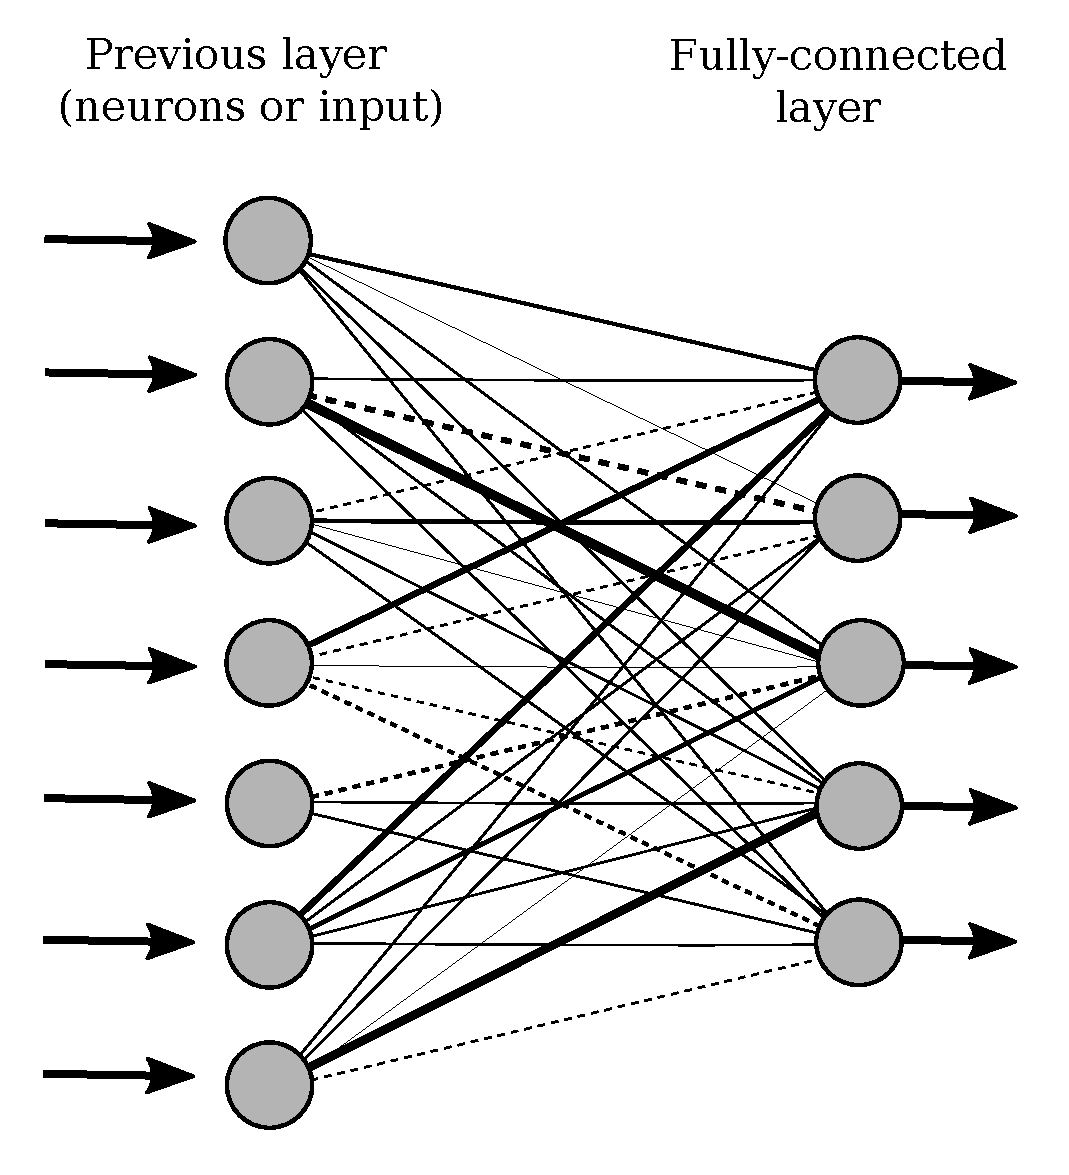
\includegraphics[width=\textwidth]{figs/fullc.pdf}
\caption{Left panel: building block of a fully-connected neural network. Each input of the previous 
layer is connected to each neuron of the output. Each connection is represent by different 
lines where the width is associated to higher weights and the dashed lines to negative weights. 
Right panel: three-dimensional convolution carried out by a convolutional layer. The 3D-kernel traverses
the whole input, producing a single scalar at each position. At the end, a 2D feature map will be 
created for each 3D kernel. When all feature maps are stacked, a feature map tensor will be created.}
\label{fig:networks}
%http://setosa.io/ev/image-kernels/
%file:///scratch/carlos/REDMOLONA/DIBUJO_CONVOL/main.py
\end{figure}

The most used type of neural network from the 1980s to the 2000s
is the fully connected network \cite[FCN; see][for an overview]{Overview2014}, 
in which every input is connected to every neuron of the following layer. Likewise, the output 
transformation becomes the input of the following layer (see left panel of Fig. \ref{fig:networks}).
This kind of architecture succeeded to solve problems that were considered to be not easily solvable as the recognition of handwritten characters \cite{B96}. A selection of applications in Solar Physics include the inversion of Stokes profiles 
\cite[e.g.,][]{socas05,carroll08}, the acceleration of the solution of chemical equilibrium \cite{asensio05}
and the automatic classification of sunspot groups \cite{colak08}.

Neural networks are optimized iteratively by updating the weights and biases so that 
a loss function that measures the ability of the network to predict the output from the input 
is minimized\footnote{This is the case of supervised training. Unsupervised neural networks
are also widespread but are of no concern in this paper.}. This optimization is widely known as 
learning or training process. In this process a training dataset is required.

The Artificial Neural Network (ANN) with one hidden layer is a universal approximant to any non-linear continuous function (e.g., Jones 1990; Blum \& Li 1991). The schematic structure of such a network is shown in Fig. 1. We have con- structed an ANN with an input layer of three neurons where the temperature, hydrogen density and electron density are in- troduced. The neurons of the input layer have a linear activa- tion function. The hidden layer consists on Nh neurons with a non-linear activation function σ(x). Each hidden neuron is con- nected to all the neurons of the input layer by a certain weight (indicated by arrows in the figure). The value obtained at each hidden neuron is a linear combination of the values at the neu- rons of the input layer multiplied by the weights. These values are then applied the non-linear function σ(x), multiplied by an- other set of weights and summed to give the final output of the neural network. The output of the network can be written as:
Nh ����
N(T,n(H),n(e),m)= vjσwTjT+wHjn(H) j��
+wejn(e)+uj , (13)
where the activation function is usually given by the sigmoid or the hyperbolic-tangent function. In this case, we have selected σ(x) = tanh(x). In the previous expression, m formally repre- sents the whole set of 5 × Nh weights which define the neural network.
\subsubsection{Multi-layer perceptron}
\subsubsection{Convolutional neural networks}

Motivated by the recent enormous success of deep neural networks 
\citep{Goodfellow2016}, we 
propose in this work to leverage DNN to carry out three-dimensional inversions 
of the solar atmosphere under the assumption of LTE for Hinode-like
observations. Our approach is termed  (standing for ).
We defer for the future the study of a neural approach
for the inversion of spectropolarimetric data at the diffraction limit of
a 4m class telescope like DKIST or EST and/or including non-LTE effects.
Data-driven approaches using DNNs have already been applied to solar
physics, demonstrating striking capabilities to solve problems that could not
be solved otherwise or with a much improved precision and/or speed. For instance, we 
managed to infer transverse velocities from pairs of consecutive 
images \cite[DeelVel;][]{Asensio2017}, which allowed us to identify 
small-scale vortices in the solar atmosphere that last for a few minutes and with
sizes of the order of a few hundred kilometers, something
impossible with methods based on local correlation tracking \cite{NovemberSimon_1988}. 
We have also applied them to
compensate for the blurring effect of the telescope and the Earth atmosphere
\cite{Enhance18,DeepMFBD18}. \cite{Illarionov18} applied DNNs for the automatic
segmentation of coronal holes with great success.
The advances in the field of deep learning suggests it is 
timely to investigate what are the prospects of neural networks in the field
of spectropolarimetric inversions. In this paper
we leverage convolutional neural 
networks \cite[CNN;][]{LeCun1998} that can easily exploit spatial information and 
the ability to train really deep neural networks that can approximate very nonlinear mappings.

Finally, we point out that the application of neural networks (multi-layer perceptrons; MLP) 
for the inversion of Stokes profiles is not
new. \cite{Carroll2001} already proposed their use for simple Milne-Eddington
inversions and concluded that they were able to obtain physical parameters
without any optimization once the neural networks were trained. As additional
advantages, they showed their speed, noise tolerance and stability. This
was later verified by other works \cite{socas_nn_03,socas_nn_05}. 
\cite{Carroll2008} later expanded their original work to use MLPs to
infer the depth stratification in a geometrical height scale of the temperature, velocity and
magnetic field vector, as their network was trained with a quiet Sun simulation \cite{vogler05}.
The application of the neural network pixel by pixel allowed them to recover
a tomographic view of the FOV by recombining all individual line-of-sight stratifications. 
More recently, \cite{osborne2019} has shown
how invertible neural networks \cite[INNs;][]{Ardizzone2018} can be successfully applied to capture 
degeneracies and ambiguities in the inference of thermodynamic parameters of
plane-parallel chromospheres of flaring regions.

\subsection{Convolutional neural networks}
In spite of the relative success of neural networks, their application to 
high-dimensional objects like images or videos turned out to be
an obstacle. The fundamental reason was that the number of
weights in a fully connected network increases extremely fast with the complexity of the network (number of neurons) and the computation quickly becomes unfeasible.
As each neuron has to be connected with the whole input, if we add a new neuron we will add the size of the input in number of weights. Then, a larger number of neurons implies a huge number of connections.
% increased dimensionality in the input
This constituted an
apparently unsurmountable handicap that was only solved with the
appearance of convolution neural networks \cite[CNN or ConvNets;][]{LeCun1998}.




The most important ingredient in the CNN is the convolutional layer which is composed of
several convolutional neurons. Each CNN-neuron carries out the convolution of the input with a certain
(typically small) kernel, providing as output what is known as feature map. Similar to a FCN, the output of
convolutional neurons is often passed through a nonlinear activation function.
The fundamental advantage of CNNs is that the same weights are shared across the whole input, 
drastically reducing the number of unknowns. This also makes
CNN shift invariant (features can be detected in an image irrespectively of
where they are located). 

%It is  convolutional layer usually works on three-dimensional volumes of 
%data (also called tensors or cubes).

In mathematical notation, for a two-dimensional input $X$
of size $N \times N$ with $C$ channels\footnote{The term channels is inherited from
the those of a color image (e.g., RGB channels). However, the term has a much more general
scope and can be used for arbitrary quantities \cite[see][for an application]{Asensio2017}.} 
(really a cube or tensor of size $N \times N \times C$), each output feature map $O_i$ (with size $N \times N \times 1$) of a convolutional layer is computed as:
\begin{equation}
O_i=K_i * X + b_i,
\end{equation}
where $K_i$ is the $K \times K \times C$ kernel tensor associated with the output feature map $i$, 
$b_i$ is a bias value ($1 \times 1 \times 1$) and the convolution is displayed with the symbol $*$. 
Once the convolution with $M$ different kernels is carried out and stacked together, the output 
$O$ will have size $N \times N \times M$. All convolutions are here indeed intrinsically three dimensional, 
but one could see them as the total of $M \times C$ two dimensional convolutions plus the 
bias (see right panel of Fig. \ref{fig:networks}).

CNNs are typically composed of several layers. This layerwise architecture exploits the 
property that many natural signals are a generated by a hierarchical composition of 
patterns. For instance, faces are composed of eyes, while eyes contain a similar internal structure. 
This way, one can devise specific kernels that extract this information from 
the input. As an example, Fig. \ref{fig:featuremap} shows the effect of a vertical border detection 
kernel on a real solar image. The result at the right of the figure is the feature map.  
CNNs work on the idea that each convolution layer extracts information about certain patterns, 
which is done during the training by iteratively adapting the set of convolutional
kernels to the specific features to locate. This obviously leads to a much more optimal solution as
compared with hand-crafted kernels. Despite the exponentially smaller 
number of free parameters as compared with a fully-connected ANN, CNNs produce much better 
results. It is interesting to note that, 
since a convolutional layer just computes sums and multiplications of the inputs, 
a multi-layer FCN (also known as perceptron) is perfectly capable of reproducing it, but it would require more 
training time (and data) to learn to approximate that mode of operation 
\cite{Peyrard15}.



%If each neuron is managing each pattern, a $N\times N$ image of circles would need $N\times N$ FCN-neurons while %now with a CNN-neuron with a circle pattern is enough to detect the circles. In this case, the kernel could be %generated to detect borders and this matrix can have positive and negative values. 
%This layerwise architecture exploits the property of many natural signals of being compositional hierarchies, in which higher-level features are obtained by composing lower-level ones. 

%CNNs are then specially designed to process such kind of data, either in the form of sequences 
%(audio or language), images, or volumetric images like videos.


Although a convolutional layer significantly decreases 
the number of free parameters as compared with a fully-connected layer, it 
introduces some hyperparameters (global characteristics of the network) to be set in 
advance: the number of kernels
to be used (number of feature maps to extract from the input), size of 
each kernel with its corresponding padding (to deal with the borders of the image)
and stride (step to be used during the convolution
operation) and the number of convolutional layers and specific architecture to 
use in the network. As a general rule, the deeper the CNN, the better the result, 
at the expense of a more difficult and computationally intensive training. CNNs
have been used recently in astrophysics for denoising images of galaxies 
\cite{schawinski17}, for cosmic string detection in CMB temperature 
maps \cite{Ciuca17}, or for the estimation of horizontal velocities 
in the solar surface \cite{Asensio2017} .

\subsection{Activation layers}
As said, the output of a convolutional layer is often passed through a non-linear function 
that is termed the activation function. Since the convolution operation is linear, this activation
is the one that introduces the non-linear character of the CNNs. Although hyperbolic
tangent, $f(x)=\tanh(x)$, or sigmoidal, $f(x)=[1+\exp(-x)]^{-1}$, activation units were originally 
used in ANNs, nowadays a panoply of more convenient nonlinearities are used. The main problem 
with any sigmoid-type activation
function is that its gradient vanishes for very large values, difficulting
the training of the network. Probably the most common activation function is 
the rectified linear unit \cite[ReLU;][]{relu10} or slight variations of it. The ReLU
replaces all negative values in the input by zero and keeps the rest untouched. This activation
has the desirable property of producing non-vanishing gradients for positive
arguments, which greatly accelerates the training.

CNNs are trained by iteratively modifying the weights and biases of the convolutional 
layers (and any other possibly learnable parameter in the activation layer). The aim
is to optimize a user-defined loss function from the output
of the network and the desired output of the training data. The optimization
is routinely solved using simple first-order gradient descent algorithms \cite[GD; see][]{Rumelhart1988}, which modifies the weights along
the negative gradient of the loss function with respect to the model parameters
to carry out the update. The gradient of the loss function with respect to the 
free parameters of the neural network is obtained through the
backpropagation algorithm \cite{LeCun1998b}. Given that neural networks are 
defined as a stack of modules (or layers), the gradient of the loss 
function can be calculated using the chain rule as the product of the 
gradient of each module and, ultimately, of the last layer and the
specific loss function.

In practice,
procedures based on the so-called stochastic gradient descent (SGD) are used, in which
only a few examples (termed batch) from the training set are used
during each iteration to compute a noisy estimation of the gradient and adjust the weights 
accordingly. Although the calculated gradient is a noisy estimation of the one calculated with the whole training set, the training is faster as we have less to compute and
more reliable. If the general loss function $Q$ is the average of each loss $Q_j$  computed on a batch of inputs and it can be written as $Q=\Sigma_j^n Q_j/n$, the weights $w_i$ are updated following the same recipe as the 
gradient descend algorithm but calculating the gradient within a single batch:
\begin{equation}
w_{i+1} = w_i -\eta\nabla Q(w_i) = w_i -\eta\nabla\Sigma_j^n Q_j(w_i)/n \simeq w_i -\eta\nabla Q_j(w_i),
\end{equation}
where $\eta$ is the so-called learning rate.
%and it determines the step size or velocity of we update the weights. 
It can be kept fixed or it can be changed according to our requirements. This parameter has to be tuned to find a compromise between the accuracy of the network and the speed of convergence. If $\eta$ is too large, the steps will be too large and the solution could 
potentially overshoot the minimum. On the contrary, if it is too small it will take so many iterations to reach the minimum. Adaptive methods like
Adam \cite{adam14} have been developed to automatically tune the
learning rate.
%https://arxiv.org/pdf/1412.6980.pdf
%https://machinelearningmastery.com/adam-optimization-algorithm-for-deep-learning/
%http://ruder.io/optimizing-gradient-descent/

%\red{As we will comment, in our procedure we have used the Adam algorithm \cite{adam14}. This algorithm is very popular in the field of deep learning because it achieves good results fast. An extra term is added multiplying the learning rate in the classic gradient descent algorithm to accelerate the convergence computing individual adaptive learning rates for different parameters (weights).}

Because of the large number of free parameters in a deep CNNs, overfitting can be 
a problem. One would like the network to generalize well and avoid any type of "memorization" of
the training set. To check for that, a part of the training set is not used during the update
of the weights but used after each iteration as validation. Desirably, the loss should
decrease both in the training and validation sets simultaneously. If overfitting occurs, the
loss in the validation set will increase.

Moreover, several techniques have been described in the literature to accelerate
the training of CNNs and also to improve generalization. Batch normalization \cite{batch_normalization15}
is a very convenient and easy-to-use technique that consistently produces large accelerations in the
training. It works by normalizing every batch to have 
zero mean and unit variance. Mathematically, the input is normalized so that:
\begin{equation}
y_i = \gamma \hat{x_i} + \beta \nonumber \\
\hat{x_i} = \frac{x_i - \mu}{\sqrt{\sigma^2 + \epsilon}},
\end{equation}
where $\mu$ and $\sigma$ are the mean and standard deviation of the inputs on the batch and
$\epsilon=10^{-3}$ is a small number to avoid underflow. The parameters $\gamma$ and $\beta$
are learnable parameters that are modified during the training.

Following the typical scheme of a residual block, there is also a shortcut connection 
between the input and the output of the block
\cite[see more information in][]{residualnetwork16,Asensio2017}, so that the input
is added to the output. Very deep networks usually
saturate during training producing higher errors than shallow networks because
of difficulties during training (also known as the degradation problem).
The fundamental reason is that the gradient of the loss function with
respect to parameters in early layers becomes exponentially small (also known as the vanishing gradient problem). Residual networks help avoid this problem obtaining state-of-the-art results without adding any extra parameter and with
practically the same computational complexity. It is based 
on the idea that if $y=F(x)$ represents the desired effect of the block on the
input $x$, it is much simpler for a network to learn the deviations from the input (or residual mapping) that it can called $R(x)=y-x$ than the full map $F(x)$, so that $y=F(x)=R(x)+x$.

\subsubsection{Loss function}
\subsubsection{Backpropagation}

\section{Heliosphere}

\section{Flare prediction}

\section{Inversion of Stokes profiles}

\subsection{Database search}
\subsection{Artificial neural networks}

\section{Image deconvolution}


\begin{acknowledgements}
Financial support by the Spanish Ministry of Economy and Competitiveness through project AYA2014-60476-P. This research has made use of NASA's Astrophysics Data System Bibliographic Services.
\end{acknowledgements}

% BibTeX users please use one of
\bibliographystyle{spbasic}      % basic style, author-year citations
%\bibliographystyle{spmpsci}      % mathematics and physical sciences
%\bibliographystyle{spphys}       % APS-like style for physics
\bibliography{biblio}   % name your BibTeX data base

% Non-BibTeX users please use
%\begin{thebibliography}{}
%
% and use \bibitem to create references. Consult the Instructions
% for authors for reference list style.
%
%\bibitem{RefJ}
% Format for Journal Reference
%Author, Article title, Journal, Volume, page numbers (year)
% Format for books
%\bibitem{RefB}
%Author, Book title, page numbers. Publisher, place (year)
% etc
%\end{thebibliography}

\end{document}
% end of file template.tex

